\documentclass{article}
\usepackage[utf8]{inputenc}
\usepackage{graphicx}

\title{Elaboration II}
\author{Sophie.Wallace }
\date{September 2019}

\begin{document}

\maketitle
\tableofcontents
\clearpage
\section{Task Outline}
After progressing through elaboration I and identifying the proposed technologies, it is now required to test these tools to see whether they can solve the predetermined pains and gains. These tools were categorised into two alternative routes. The first included two different software packages called \textbf{Open Semantic Search} and \textbf{Tropy}. Whilst the second utilises \textbf{Micrsoft Excel}, a traditional offline tool that will be combined with the \textbf{cloudstor sync client} (CSC). Through this second elaboration I am hoping to achieve a desired outcome of uncovering whether these tools can resolves the pains from the scoping exercise and achieve criteria specified in the previous elaboration.


\section{Elaboration Tests}
To examine these tools, individual components required for this POC will be tested to see if they meet user expectations. Each component will be run individually to document validity and credibility. Recording of these tests will be completed in my learning journal, however outcomes will be discussed below. The key questions that will orient the tests include:
\begin{itemize}
\item Is this tool compatible with all data types?
\item Does this tool organise files with rich metadata?
\item Does this tool allow for editing of data?
\item Can this tool operate offline?
\item Does this tool have a reliable storage system?
\item Is this tool compatible with both mobile and desktop?
\end{itemize}
\clearpage
\section{Outcomes}
\subsection{Open Semantic Search}
Open Semantic Search had many difficulties in the downloading process. Although determined to be a useful application that met specified criteria, many problems were encountered in trying to get the application to run. Firstly, VirtualBox needed to be downloaded and installation failed twice. I then consulted with Brian and had to alter my system preferences to allow for successful installation. After installation, I realised I had only downloaded one component and needed to download the open semantic search program. The estimated time was 2 hours and never went down, therefore I switched to testing another software program that I quickly found called DEVONthink 3. Tests were able to be succesfully run and the outcomes for DEVONthink 3 are below in subsection 3.3. \\
\\
\\
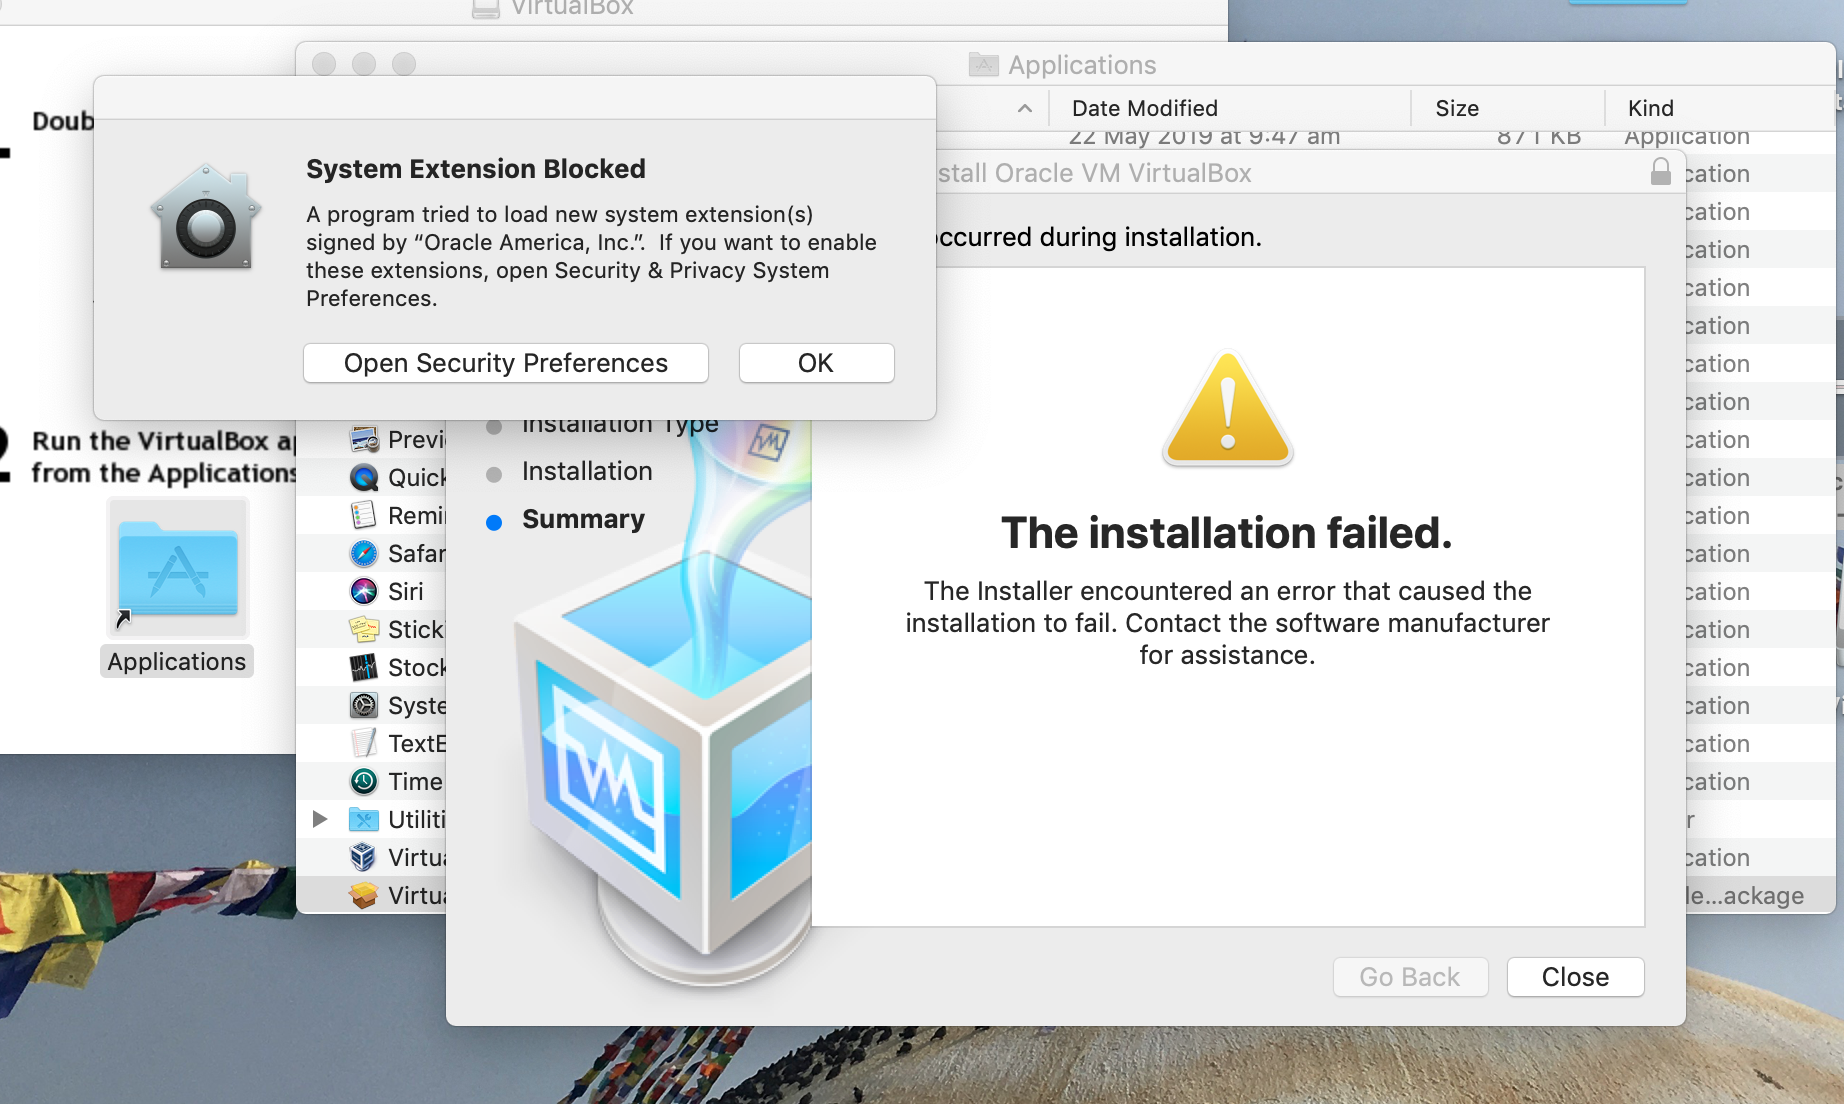
\includegraphics[width=\textwidth]{OpenSemanticSearch.png} 

\clearpage
\subsection{Tropy}
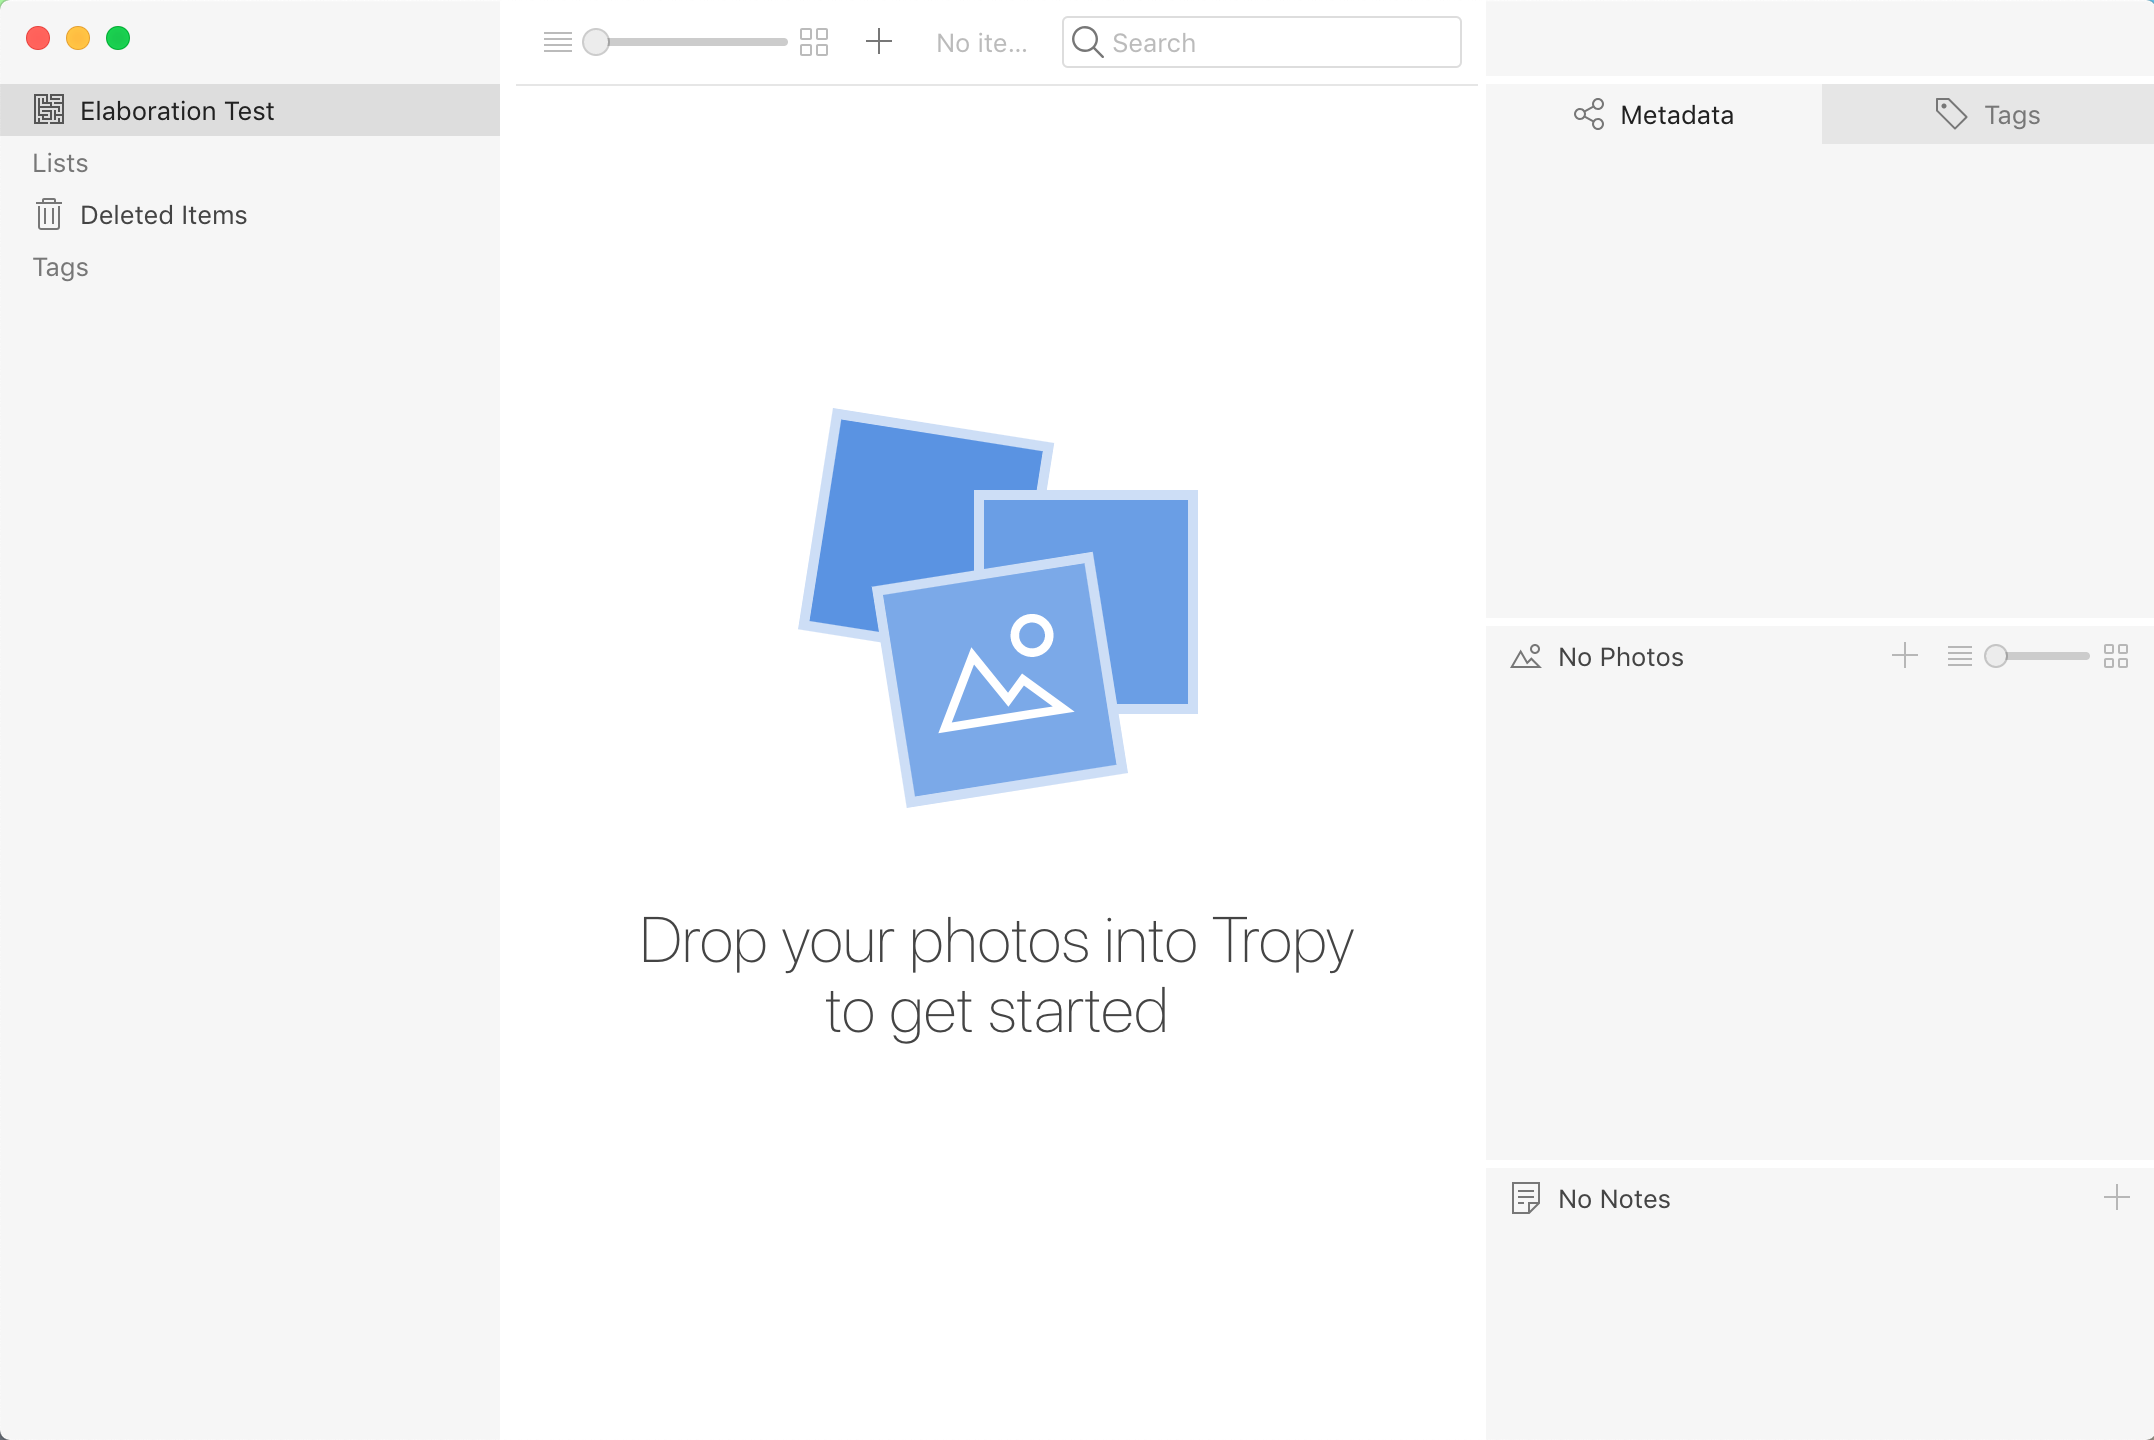
\includegraphics[width=\textwidth]{TropyInterface.png}
\\
Tropy was downloaded with ease. Its user interface was clean and manageable and the drag and drop method of uploading data was efficient and quick. There were varied outcomes through the test that will be discussed in the subsections below. 

\subsubsection{Data Type Compatibility}
The lack of data type compatibility was Tropy's major downfall. Tropy only functions for photographs. All tests in uploading other data types encountered errors and were unsuccessful. Despite this, the uploading of photos quick and efficient. 
\subsubsection{Metadata and Management}
Adding metadata to the images was extensive in Tropy. A section is clearly named and indicated for metadata, which allows rich metadata to be recorded such as sections for title, creator, date, type, archive, collection, description and notes. There is also an additional tagging section where you can organise photos according to their tagged area. This allowed for rich metadata to be recorded and data to be organised efficiently. Sections of the photo can also be selected for additional metadata on a specific area or subject in the photo. 
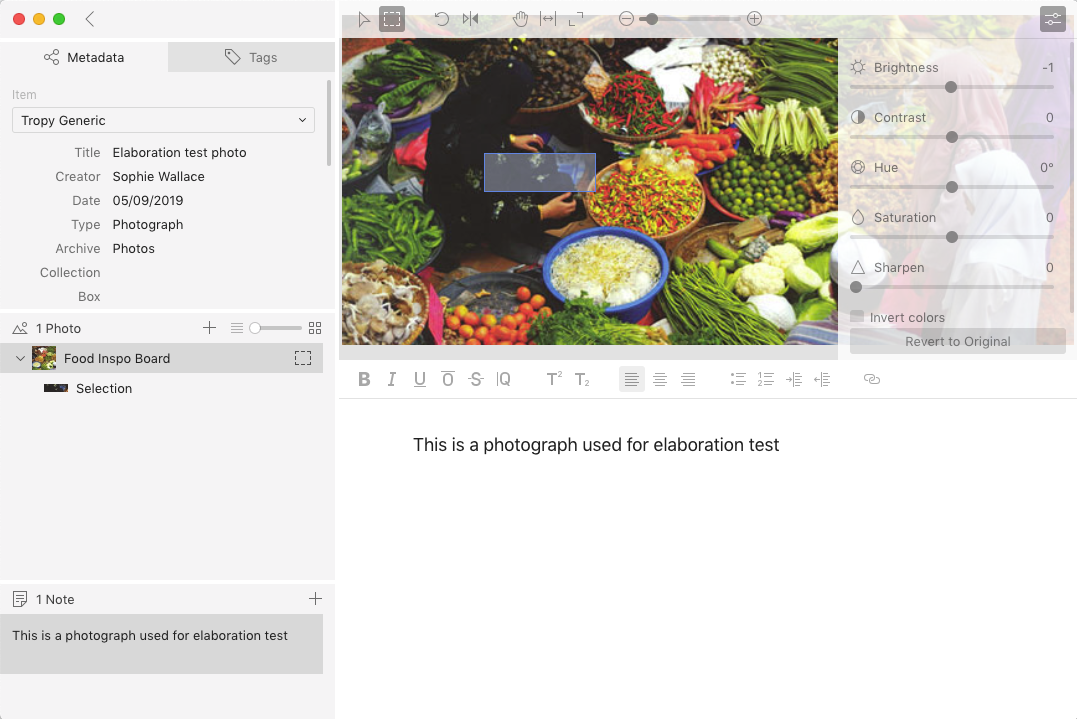
\includegraphics[width=\textwidth]{TropyMetadata.png}
\subsubsection{Editing Format}
The editing format for Tropy was inbuilt and allowed for photo aesthetics to be edited such as brightness, contrast, hue, saturation, sharpen and cropping. 
\subsubsection{Offline Operation}
Tropy was able to be used whilst offline. All functions were still applicable.
\subsubsection{Storage System}
Upon searching the interface of the application I was unable to find the syn option for Tropy. However there was an option on the website browser to sync with GitHub therefore Tropy has access to a safe and reliable storage system.
\subsubsection{Mobile and Desktop Compatibility}
I was unable to find a mobile application for Tropy. When searching for Tropy on my mobile browser, the download function was unable to be accessed therefore I concluded that Tropy is not compatible with mobile. 

\subsection{DEVONthink 3}
DEVONthink 3 was an alternative route identified after failing to download open semantic system. Its download process happened within 5 minutes. DEVONthink 3 met the most criteria that was specified in this elaboration, however there are inbuilt costs. It's user interface is also cluttered with many features therefore to understand its potential will take time and practice.
\subsubsection{Data Type Compatibility}
All data types were able to be successfully uploaded into the application. This was done with a drag and drop method into the user interface and was quick and efficient. Each data type was uploaded as its own file and was able to be reopened into its own application. This application had the best compatibility with all data types.
\subsubsection{Metadata and Management}
Extensive metadata was able to be recorded with all uploaded data files. This included the name of the file, its date added and date modified, the size, kind, location and description. Tags are also provided to categorize data therefore management of files is organized. 
\subsubsection{Editing Format}
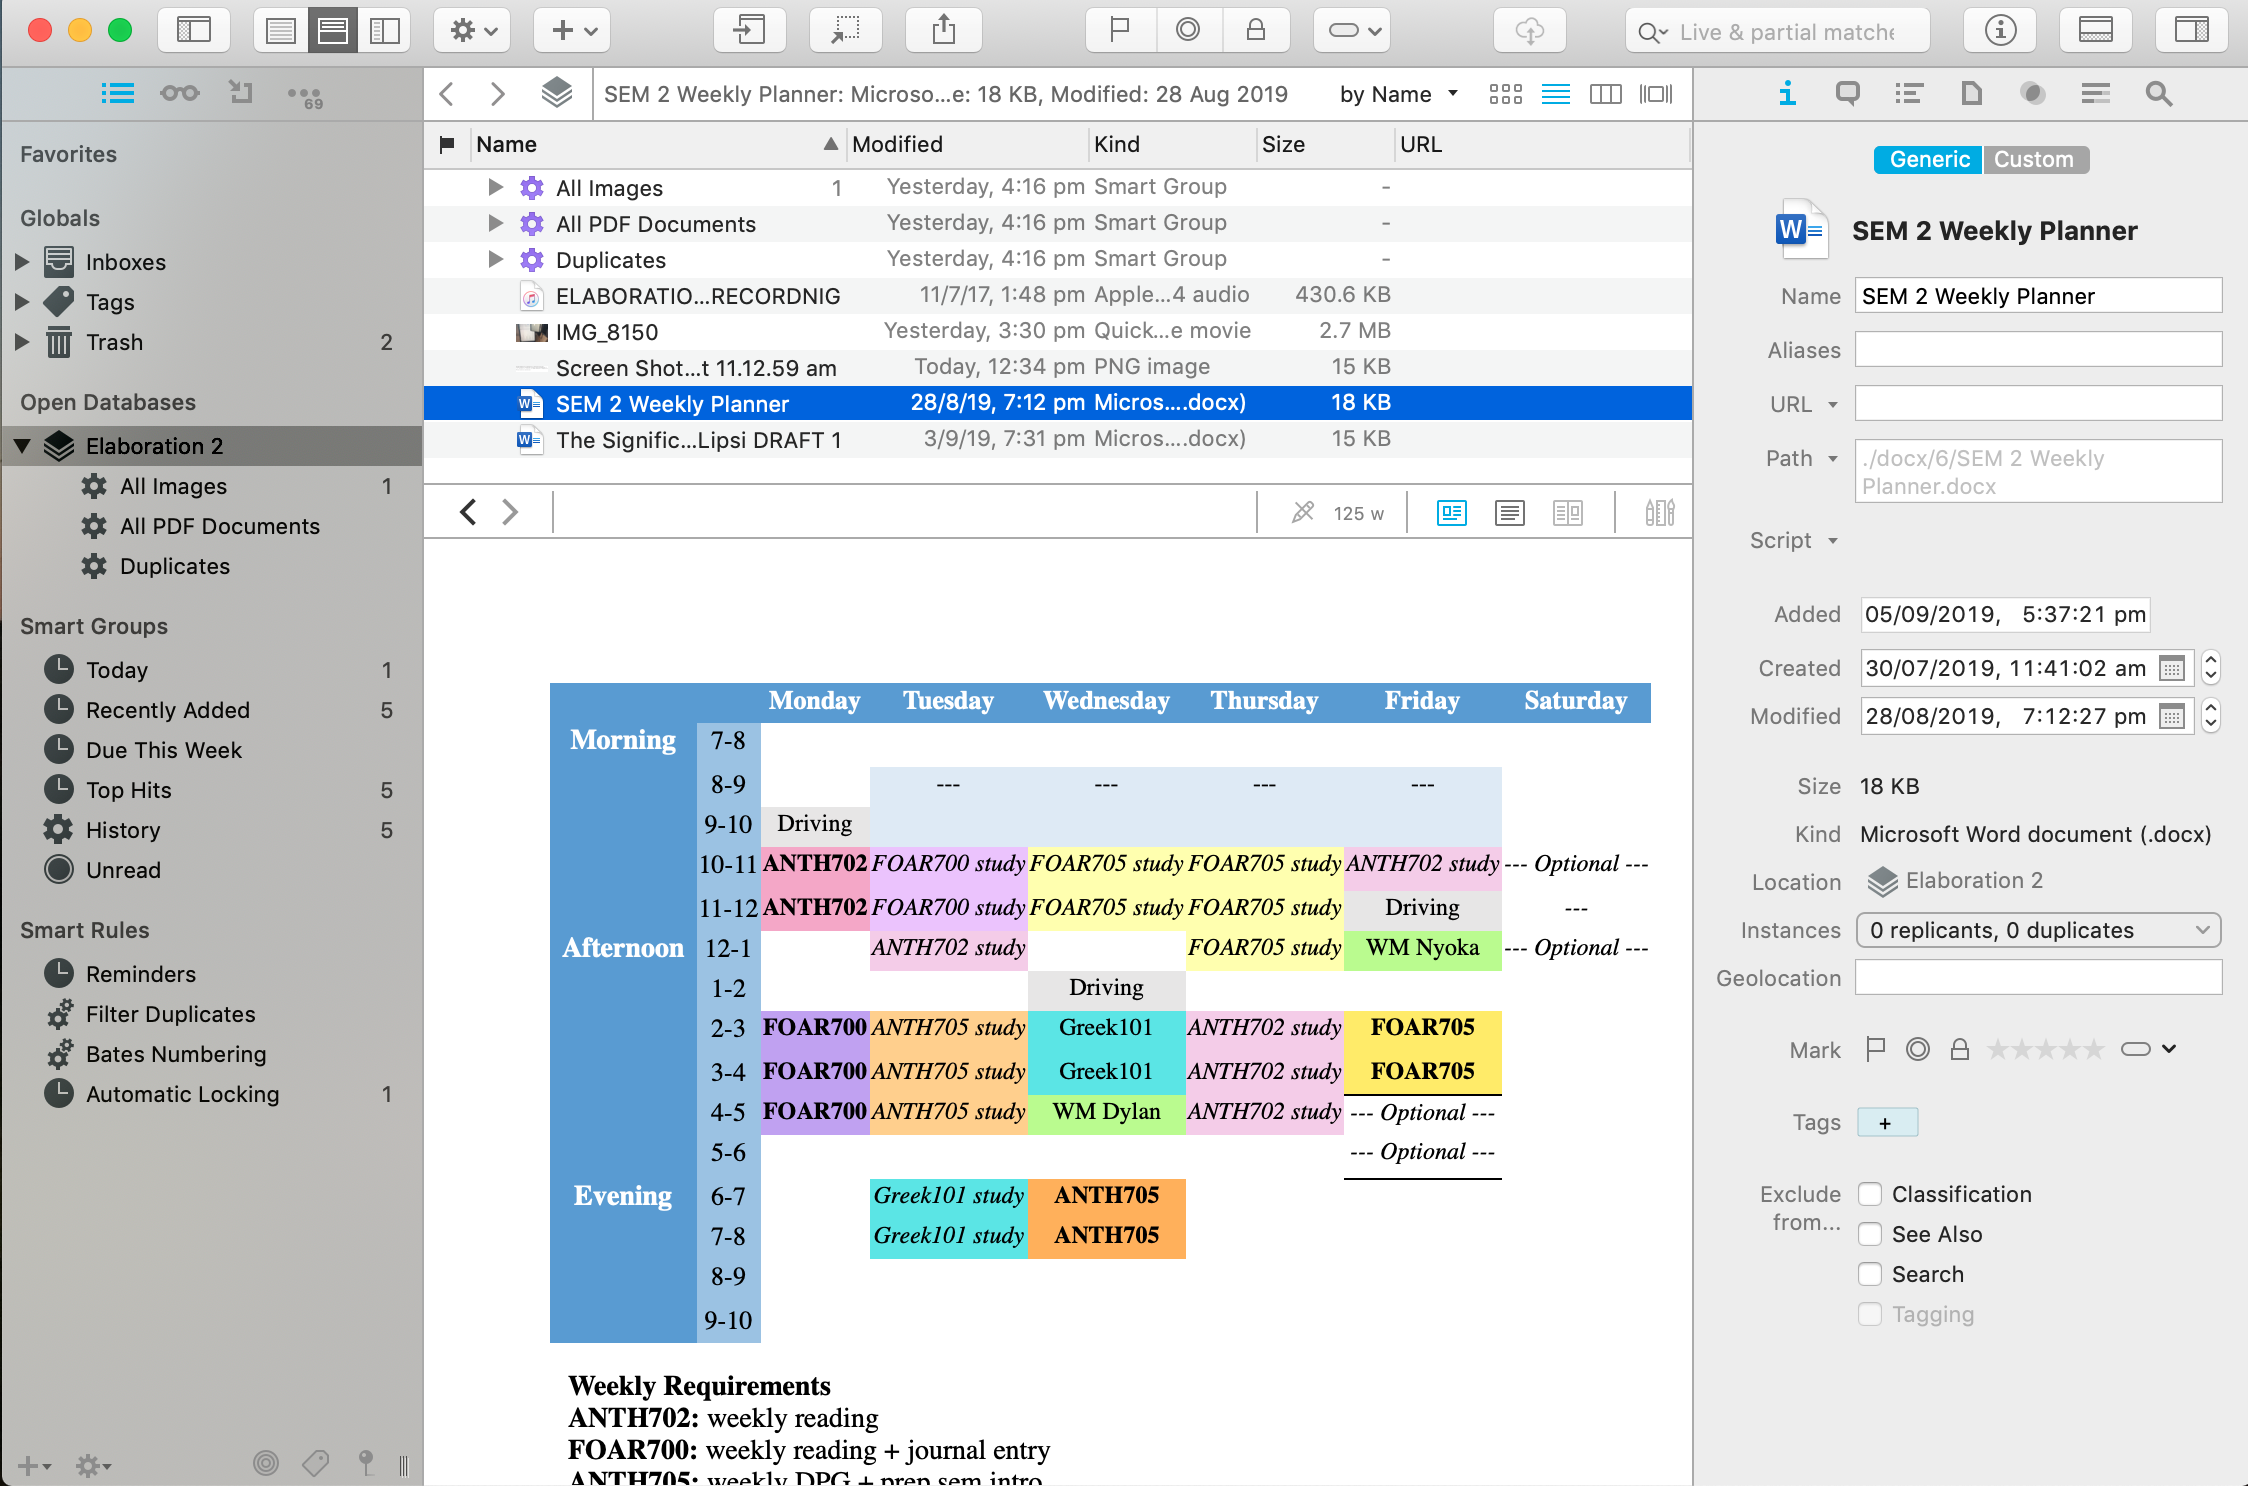
\includegraphics[width=\textwidth]{DevonInterface.png}
The editing features in DEVONthink 3 were the most extensive. Double clicking on image and text files provided the option for editing and modifying files. Images were able to have basic colour corrections, cropping, and text boxes and visual effects added. Text documents were able to be viewed in different formats. with the editing format permitting text, font, size and paragraph alterations. Word count was also included.
\subsubsection{Offline Operation}
DEVONthink 3 worked efficiently offline, with uploading, editing and saving all operating without an internet connection.
\subsubsection{Storage System}
This application has numerous sync options. Therefore data can be successfully stored in a chosen sync client. 
\subsubsection{Mobile and Desktop Compatibility}
DEVONthink 3 has a mobile application and syncs data between both mobile and desktop.

\subsection{Excel + CloudStor Client Sync}
Excel + Cloudstor Client Sync (CSC) was already loaded on the laptop and provided an alternative route to already established software packages. Although download was unnecessary, the management of excel required a lot of technical debt due to the manual labour required to organise. Tests had a variety of outcomes for the specified criteria.
\subsubsection{Data Type Compatibility}
Uploading data types such as image, video and audio files were a success. However, text files and word documents were unable to be uploaded. Although images, video and audio files were uploaded with ease, once in excel their compatibility was messy and inconsistent.
\subsubsection{Metadata and Management}
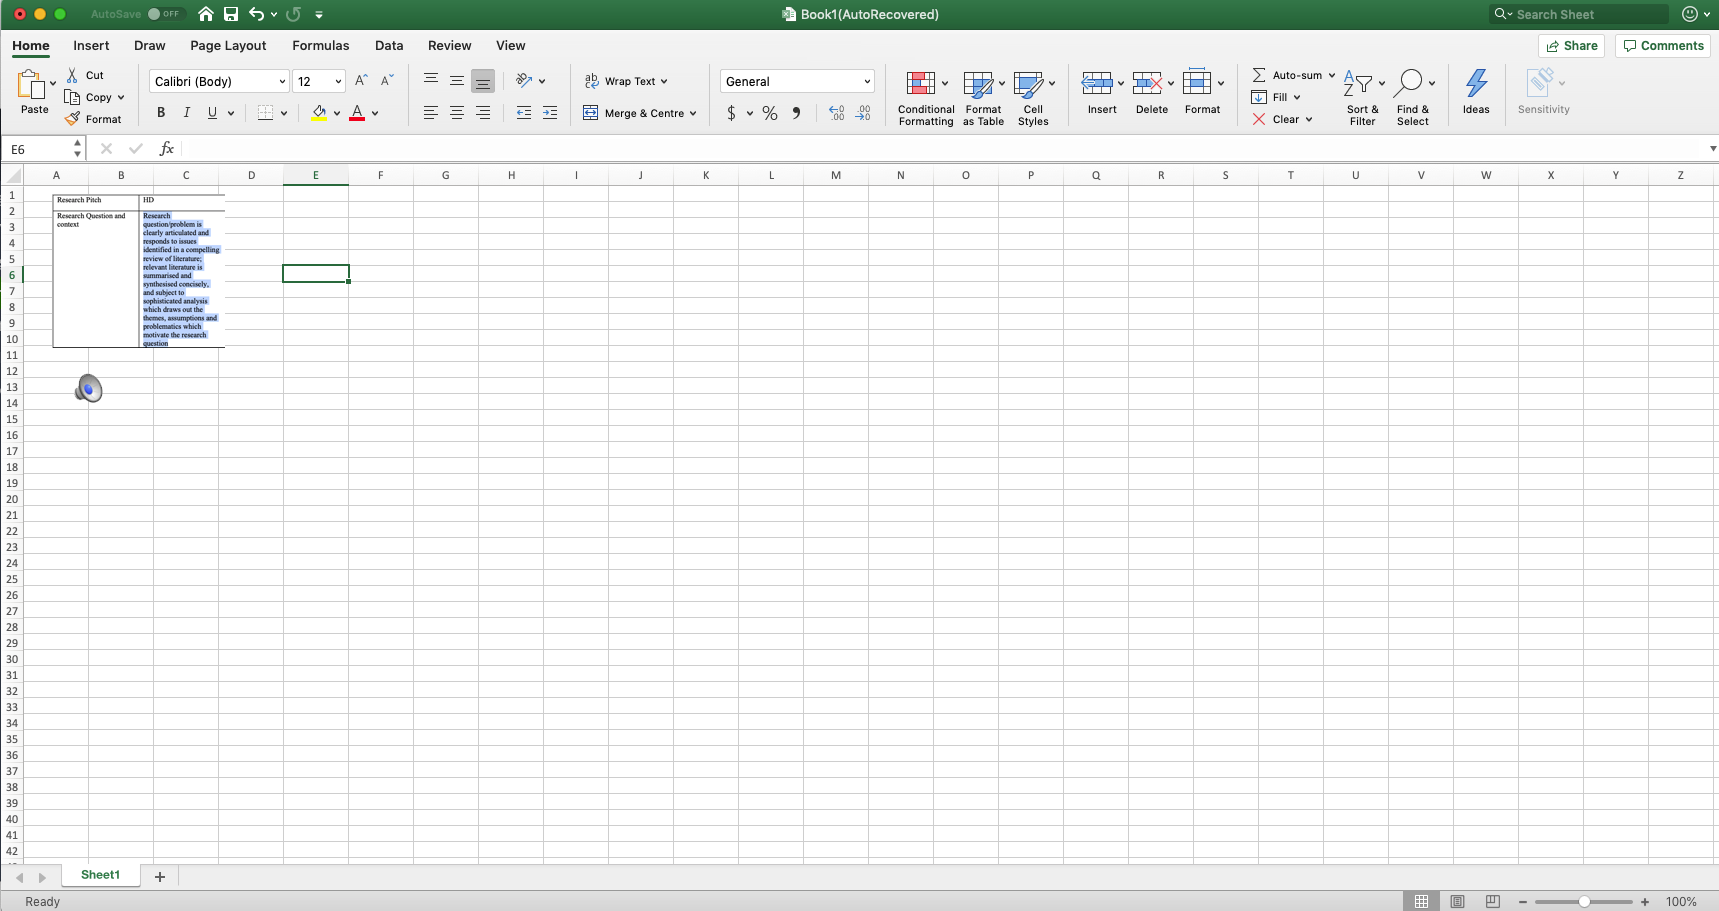
\includegraphics[width=\textwidth]{Excel_Interface.png}
Excel exceeds in its ability to manually entered endless categories and extensive metadata. However, the management of individual data files within the application was unsuccessful and tedious. This proved to involve the most technical debt out of all applications due to the lack of automation in organising metadata and data. 
\subsubsection{Editing Format}
An editing tab appeared when double clicking on the image file in excel. However options were minimal and no other data files were able to be modified. 
\subsubsection{Offline Operation}
All functions of excel were able to be utilised when offline. 
\subsubsection{Storage System}
The storage system for this application was in conjunction with CSC and the test was deemed inconclusive. Installing CSC was a straightforward process however accessing CSC was challenging. After gaining access, 13GB of CloudStor files were syncing to my computer and I therefore paused the syncing process. After saving workbook in allocated CSC folder, the file did not appear in the CloudStor browser. Although inconclusive, I did not think that additional tests were needed for this tool as previous tests displayed its insufficiency in meeting criteria.
\subsubsection{Mobile and Desktop Compatibility}
Microsoft Excel has a mobile application that would create transformation of data to desktop relatively easy.

\section{Results}
Through running these elaboration tests, the desired tools and techniques required for the eventual POC demonstration have been identified. In testing \textbf{open semantic search}, it became clear that the download process of the eventual POC must be straightforward and easily accessed for users to be satisfied. Testing \textbf{Tropy} identified numerous pain solutions and gain creators discussed in the scoping exercise. Tropy allowed for efficient uploading of files and automated categorization. The metadata section of Tropy was the most useful and relevant to this desired POC. Additionally having designated sync client such as GitHub allows for safe and reliable storage as well as version control. Thereafter the alternative solution of \textbf{DEVONthink 3} displayed the vast compatibility that software programs can have with varied data sets. Similarly, its compatibility with mobile and desktop allows for data to be transferred with ease. This tool displayed the most appropriate functions for the specified criteria, however its complicated interface and possible additional costs may provide challenges and risks. In testing \textbf{Excel + CSC}, I was able to decide that this tool would not be useful for the eventual POC demonstration. This is due to the technical debt it acquires through manual metadata formatting, which is a pain I am trying to solve. These results implicate that my eventual POC would have an interface and metadata function similar to Tropy, whilst utilizing the data and mobile compatibility, as well as the editing format, of DEVONthink 3. A syncing client applied to the POC will be similar to both Tropy and DEVONthink 3. Utilisation of cloudstor and github would be ideal.

\end{document}